\title{Assignment 2: CS 763, Computer Vision}
\author{}
\date{Due: 17th February before 11:55 pm}

\documentclass[11pt]{article}

\usepackage{amsmath}
\usepackage{amssymb}
\usepackage{hyperref}
\usepackage{ulem}
\usepackage{fancyvrb}
\usepackage{todonotes}

\usepackage[margin=0.5in]{geometry}
\usepackage{subfig}

\begin{document}
\maketitle

\textbf{Remember the honor code while submitting this (and every other) assignment. All members of the group should work on all parts of the assignment. We will adopt a \textbf{zero-tolerance policy} against any violation.}
\\
\\
\textbf{Submission instructions:} You should ideally type out all the answers in Word (with the equation editor) or using Latex. In either case, prepare a pdf file. Put the pdf file and the code for the programming parts all in one zip file. The pdf should contain the names and ID numbers of all students in the group within the header. The pdf file should also contain instructions for running your code. Name the zip file as follows: A2-IdNumberOfFirstStudent-IdNumberOfSecondStudent-IdNumberOfThirdStudent.zip. (If you are doing the assignment alone, the name of the zip file is A1-IdNumber.zip). Upload the file on moodle BEFORE 11:55 pm on 17th February. Late assignments will be assessed a penalty of 25\% per day late. Note that only one student per group should upload their work on moodle. Please preserve a copy of all your work until the end of the semester. 

\begin{enumerate}
\item Prove that collinearity of points is preserved under perspective projection. \textsf{[4 points]} 

\begin{itemize}
\item[Ans.] Let $P_1,P_2$ be two points on the line \[
\frac{X}{k}+l = \frac{Y}{m}+n = Z.
\]
where $k,l,m,n$ are constants for a given line and $p_1,p_2$ be their respective images through perspective projection.
 We'll show that slope of line formed by $p_1,p_2$ depends only on parameters of line which will then imply that slope will remain same for another pair $p_2,p_3$ formed by $P_2,P_3$ where $P_3$ is also a point on given $3D$ line. 


Slope of line formed by $p_1,p_2$ is 
\begin{align}
\frac{x_2-x_1}{y_2-y_1} &= \frac{\frac{f X_2}{Z_2}-\frac{f X_1}{Z_1}}{\frac{f Y_2}{Z_2}-\frac{f Y_1}{Z_1}} \\ 
 &= \frac{X_2 Z_1 - X_1 Z_2}{Y_2 Z_1 - Y_1 Z_2} \\ 
 &= \frac{k(Z_2-l)Z_1 - k(Z_1-l)Z_2}{m(Z_2-n)Z_1 - m(Z_1-n)Z_2}\\
 &= \frac{kl(Z_2-Z_1)}{mn(Z_2-Z_1)}\\
 &= \frac{kl}{mn}
\end{align}
which depends only on parameters of the line implying that slope of $p_2,p_3$ will be same and $p_1,p_2,p_3$ are collinear if $P_1,P_2,P_3$ are collinear.

Thus proven that linearity is preserved under perspective projection.
\end{itemize}

\item \textit{We have defined the concept of the Shannon entropy in class. Given a discrete random variable $X$ having probability mass function $P(X) = (p_1, p_2, ..., p_N)$, prove that $H(X) \geq 0$ where $H(X)$ is the Shannon entropy of $X$. Recall that $H(X) = -\sum\limits_{i=1}^N p_i \log p_i$ and that $\sum\limits_{i=1}^N p_i = 1$ and $\forall i, 0 \leq p_i \leq 1$. Also prove that a uniform distribution (\textit{ie} $\forall i, \textrm{ } p_i = \frac{1}{N}$) maximizes the Shannon entropy. To this end, find a stationary point of $J(X) = H(X) - \lambda (\sum\limits_{i=1}^N p_i - 1)$ where $\lambda$ is a Lagrange multiplier to impose the hard constraint that the probabilities all sum up to 1.  \textsf{[2+4 = 6 points]}}

\begin{itemize}
\item[Ans.] Note that $0 \leq p_i \leq  \forall i$ and therefore $log p_i<0$. Thus  \[
H(X) = -\sum\limits_{i=1}^N p_i \log p_i
 = \sum\limits_{i=1}^N p_i (-\log p_i)
 \geq 0
\]

To find the point of maximum of $H(X) = -\sum\limits_{i=1}^N p_i \log p_i$ given constraint  $\sum\limits_{i=1}^N p_i = 1$, we need to find the stationary point of Lagrangian $J(X) = H(X) - \lambda (\sum\limits_{i=1}^N p_i - 1)$ 


Thus $\forall i = 1 \dots N $,
\begin{align}
\frac{\partial J}{\partial p_i} = 0 \\
-\log p_i - 1 + \lambda  = 0 \\ 
p_i = 2^{\lambda -1} = \nu
\end{align}
for some constant $\nu$. Putting this back in the constraint,
\[
 \sum\limits_{i=1}^N p_i = 1
\]
we get $p_i = \nu = 1/N $  $\forall i = 1\dots N$. Thus maximum entropy for a discrete random variable is achieved at unifrom distribution.
\end{itemize}

\item This is a straightforward exercise to make sure you understand the basic update equations in the Horn-Shunck algorithm for optical flow. As seen in class, we seek to minimize the quantity $J(\{(u_{ij},v_{ij})\})$ w.r.t. the optical flow vectors $(u_{i,j},v_{i,j})$ at all pixels $(i,j)$, where $J(\{(u_{i,j},v_{i,j})\}) = \sum\limits_{i=1}^N \sum\limits_{j=1}^N (I_{x;i,j} u_{i,j} + I_{y;i,j} v_{i,j} + I_{t;i,j} )^2 + \lambda ((u_{i,j+1} - u_{i,j})^2 + (u_{i+1,j} - u_{i,j})^2 + (v_{i,j+1} - v_{i,j})^2 + (v_{i+1,j} - v_{i,j})^2)$. Setting the partial derivatives w.r.t. $u_{k,l}$ and $v_{k,l}$ to 0, prove that 
\begin{eqnarray}
u_{k,l} = \bar{u}_{k,l} - \dfrac{I_{x;k,l} (I_{x;k,l} \bar{u}_{k,l} + I_{y;k,l} \bar{v}_{k,l} + I_{t;k,l})}{I^2_{x;k,l} + I^2_{y;k,l} + 4 \lambda} \\ 
v_{k,l} = \bar{v}_{k,l} - \dfrac{I_{y;k,l} (I_{x;k,l} \bar{u}_{k,l} + I_{y;k,l} \bar{v}_{k,l} + I_{t;k,l})}{I^2_{x;k,l} + I^2_{y;k,l} + 4 \lambda}
\end{eqnarray}
where $\bar{u}_{k,l}$ and $\bar{v}_{k,l}$ are as defined in the lecture slides. \textsf{[4 points]}

\begin{itemize}
\item[Ans.] 
We have
\begin{multline*}
J(\{(u_{i,j},v_{i,j})\}) = \sum\limits_{i=1}^N \sum\limits_{j=1}^N (I_{x;i,j} u_{i,j} + I_{y;i,j} v_{i,j} + I_{t;i,j} )^2 \\
+ \lambda ((u_{i,j+1} - u_{i,j})^2 + (u_{i+1,j} - u_{i,j})^2 + (v_{i,j+1} - v_{i,j})^2 + (v_{i+1,j} - v_{i,j})^2)
\end{multline*}

Set partial derivative of J w.r.t. $u_{k,l}$ to 0 i.e $\frac{\partial J}{\partial u_{k,l}} = 0$.
In the summation above, terms which contain $u_{k,l}$ correspond to $i=k,j=l$ and $i=k-1,j=l$. On simplifying the equation, we get
\[
(I_{x;k,l}^2 + 4 \lambda) u_{k,l} + I_{x;k,l} I_{y;k,l} v_{k,l} = 4 \lambda \bar{u}_{k,l} - I_{x;k,l} I_{t;k,l}
\]

where $\bar{u}_{k,l}$ = (${u}_{k+1,l}$+${u}_{k,l}$+${u}_{k,l}$+${u}_{k,l-1}$)/4. 

Similarly setting partial derivative of J w.r.t. $v_{k,l}$ to 0 gives us
 \[
 (I_{y;k,l}^2 + 4 \lambda) v_{k,l} + I_{x;k,l} I_{y;k,l} u_{k,l} = 4 \lambda \bar{v}_{k,l} - I_{y;k,l} I_{t;k,l}
\] 
where $\bar{v}_{k,l}$ = (${v}_{k+1,l}$+${v}_{k,l}$+${v}_{k,l}$+${v}_{k,l-1}$)/4.

Solving these two equations for ${u}_{k,l}$ and ${v}_{k,l}$ gives us
\begin{align}
u_{k,l} &= \bar{u}_{k,l} - \dfrac{I_{x;k,l} (I_{x;k,l} \bar{u}_{k,l} + I_{y;k,l} \bar{v}_{k,l} + I_{t;k,l})}{I^2_{x;k,l} + I^2_{y;k,l} + 4 \lambda} \\
v_{k,l} &= \bar{v}_{k,l} - \dfrac{I_{y;k,l} (I_{x;k,l} \bar{u}_{k,l} + I_{y;k,l} \bar{v}_{k,l} + I_{t;k,l})}{I^2_{x;k,l} + I^2_{y;k,l} + 4 \lambda}
\end{align}

\end{itemize}

\item You know that both the Horn-Shunck as well as Lucas-Kanade methods bank on the brightness constancy assumption. Given a pair of images, let us suppose that this assumption holds good for most physically corresponding pixels, but not for some $p \%$ of the pixels. Briefly explain how you will modify the Horn-Shunck method and Lucas-Kanade method to deal with this. \textsf{[4 points]}
\begin{itemize}
\item[Ans.] One alternative is to use $\mathcal{L}_1$ norm instead of $\mathcal{L}_2$ norm, so as to allow for more outliers. In this scheme, 
\begin{description}
\item[Horn-Shunck] will minimise the following cost function:\begin{multline}
J(\{(u_{i,j},v_{i,j})\}) = \sum\limits_{i=1}^N \sum\limits_{j=1}^N |I_{x;i,j} u_{i,j} + I_{y;i,j} v_{i,j} + I_{t;i,j} | \\
+ \lambda ((u_{i,j+1} - u_{i,j})^2 + (u_{i+1,j} - u_{i,j})^2 + (v_{i,j+1} - v_{i,j})^2 + (v_{i+1,j} - v_{i,j})^2)
\end{multline}

\item[Lucas-Kanade] will solve the following optimization problem for each window
\[
\min \| Au - b\|_1
\]
where $A$ and $b$ are defined as in standard Lucas-Kanade method.
\end{description}

Another alternative is to use M-estimator type of function discussed in the class for penalising brightness constancy equation.
Let $f(x) = \sum_i \rho(x_i)$ where $\rho(x_i) = x_i^2$ if $|x_i|<T$ and $T^2$ otherwise. In this case, each of the methods will look like following:
\begin{description}
\item[Horn-Shunck] will minimise the following cost function:\begin{multline}
J(\{(u_{i,j},v_{i,j})\}) = \sum\limits_{i=1}^N \sum\limits_{j=1}^N f(I_{x;i,j} u_{i,j} + I_{y;i,j} v_{i,j} + I_{t;i,j}) \\
+ \lambda ((u_{i,j+1} - u_{i,j})^2 + (u_{i+1,j} - u_{i,j})^2 + (v_{i,j+1} - v_{i,j})^2 + (v_{i+1,j} - v_{i,j})^2)
\end{multline}

\item[Lucas-Kanade] will solve the following optimization problem for each window
\[
\min f( Au - b)
\]
\end{description}

\end{itemize}

\item In this assignment, you will build up on the previous assignment to estimate the homography between two images. This time, you should use the RanSaC algorithm to estimate the homography in order to make the estimate resistant to the presence of incorrect point correspondences. The code for RanSaC for various problems including estimation of homographies is available at \url{http://www.csse.uwa.edu.au/~pk/research/matlabfns/}. You should work with the images in the folder \url{http:\\www.cse.iitb.ac.in/~ajitvr/CS763_Spring2015/HW2/Homography} and also on any one pair of pictures of an approximately planar scene taken with a real camera. (You should acquire these images yourself and make sure they have small non-overlapping areas to make this more interesting.) Also, in each case, you should warp one of the images so that it aligns with the other one. However, this time you should \emph{not} crop the image so that no parts of either image are deleted, and a true mosaic may be obtained. While you should use the RanSaC code as is, I recommend stepping through it to get a feel for what is going on inside. Display all the resulting mosaics in your report. State the number of iterations and all thresholds you used. \textsf{[5 points]}
\begin{itemize}
\item[Ans.] Please refer to Figures 1,2,3 for images. Threshold used for RanSac is 0.005. 
\begin{figure}[!htb]
    \centering
    \subfloat[Image 1]{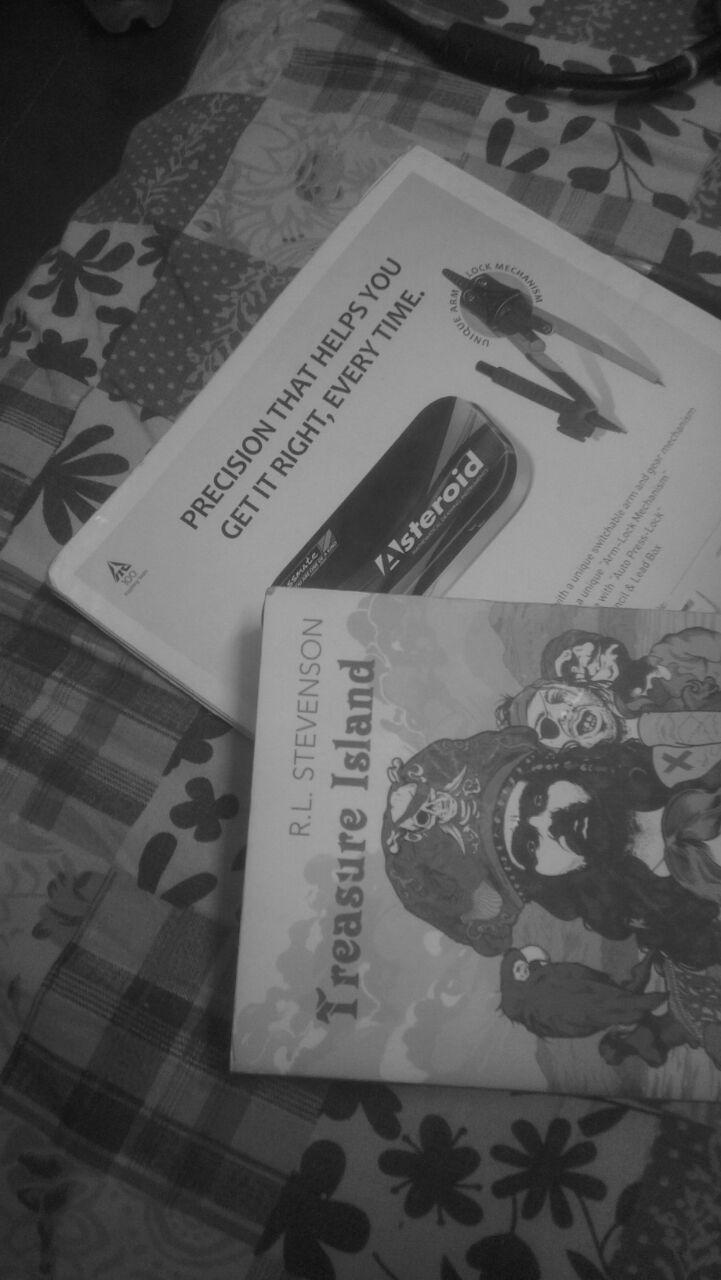
\includegraphics[width=2.5in]{test1.jpg}}%
    \qquad
    \subfloat[Image 2]{{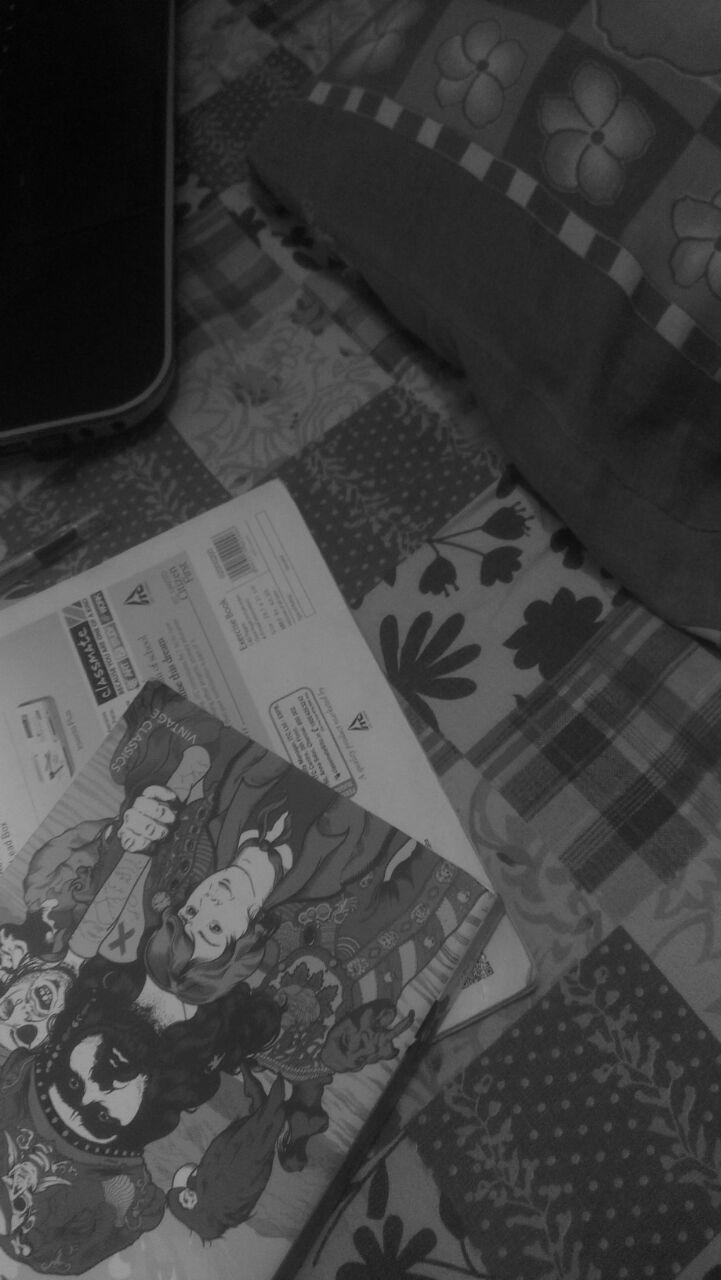
\includegraphics[width=2.5in]{test2.jpg} }}%
	\qquad
	\subfloat[Mosaiced Image]{{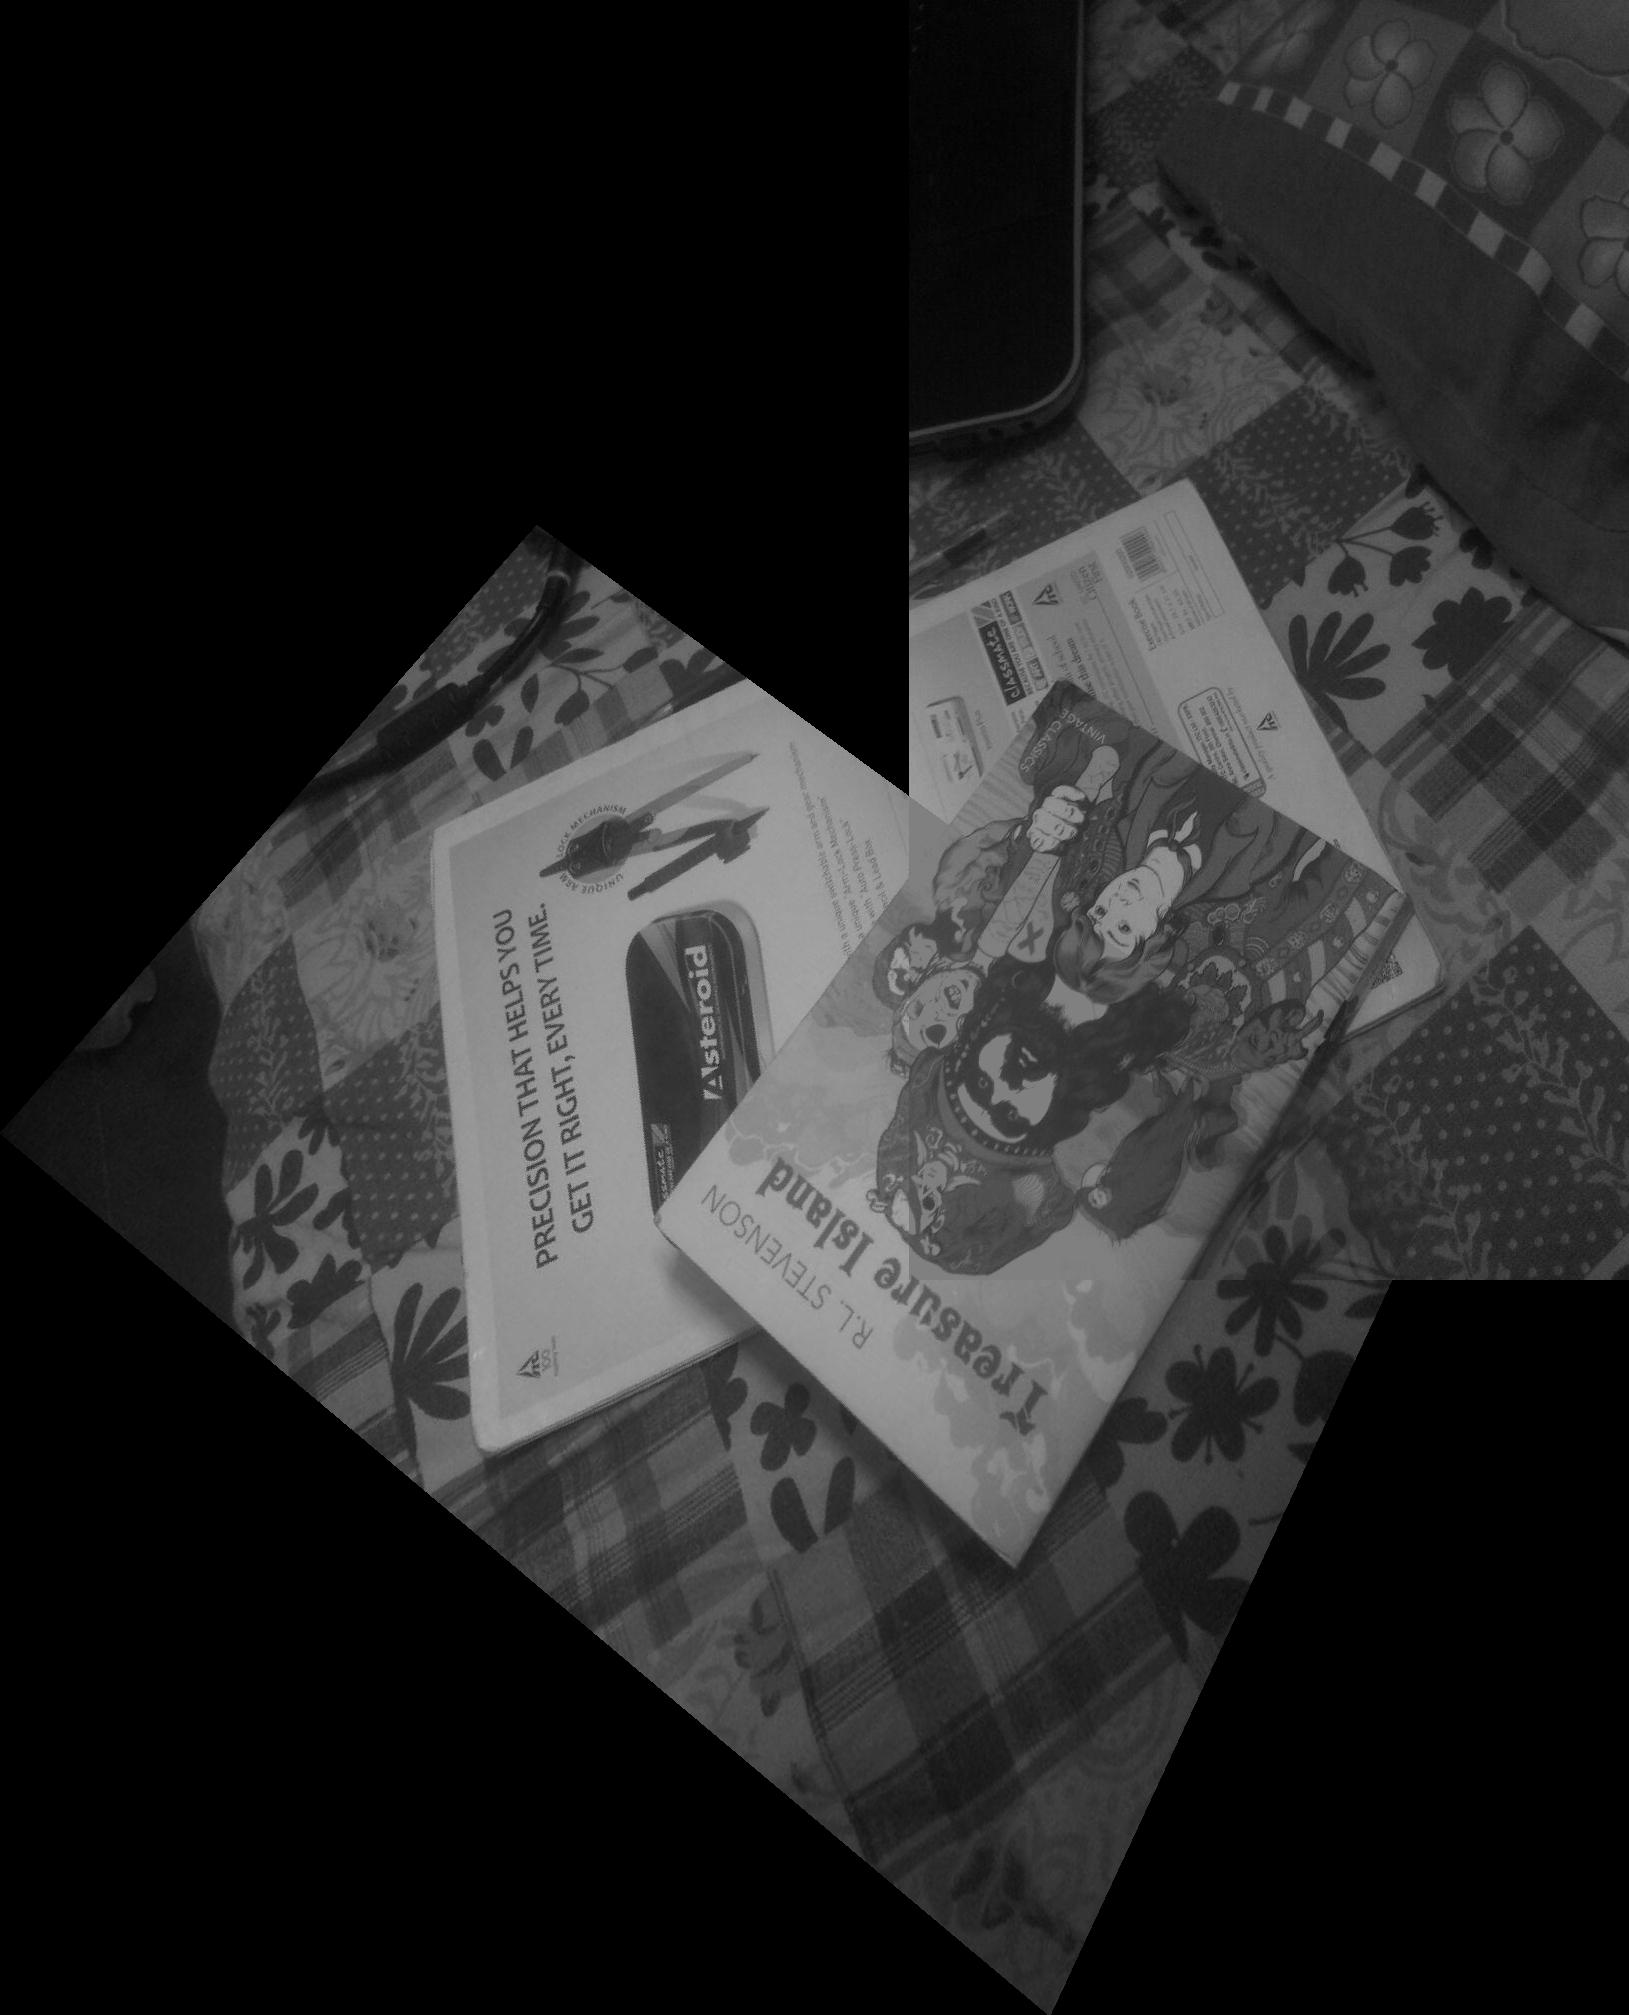
\includegraphics[width=3.5in]{test_result.jpg} }}%
	\caption{Mosaicing of my images}
\end{figure}

\begin{figure}[!htb]
    \centering
    \subfloat[Image 1]{
\includegraphics[width=2.5in]{new1.jpg}}%
    \qquad
    \subfloat[Image 2]{{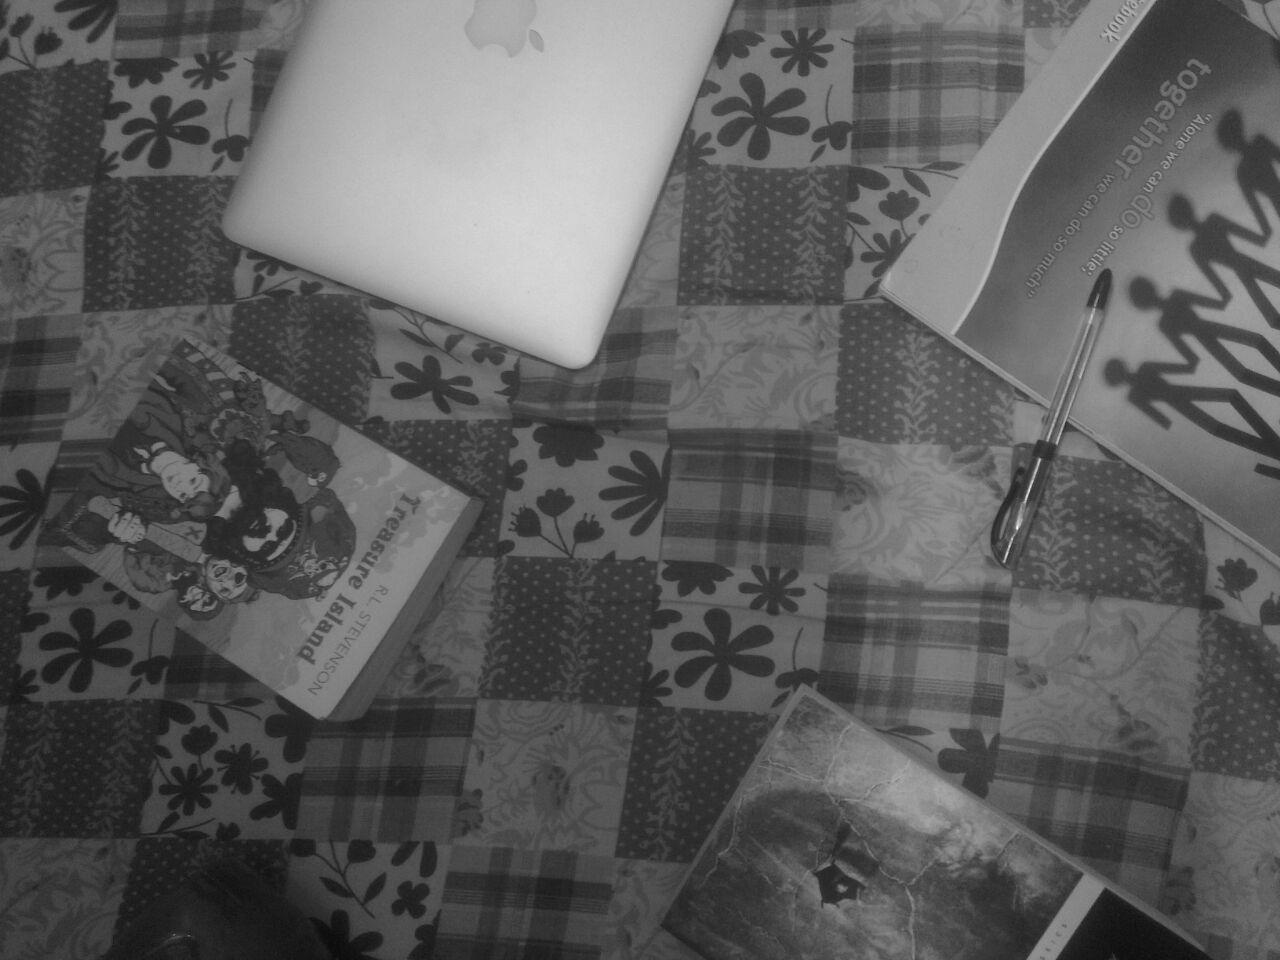
\includegraphics[width=2.5in]{new2.jpg} }}%
	\qquad
	\subfloat[Mosaiced Image]{{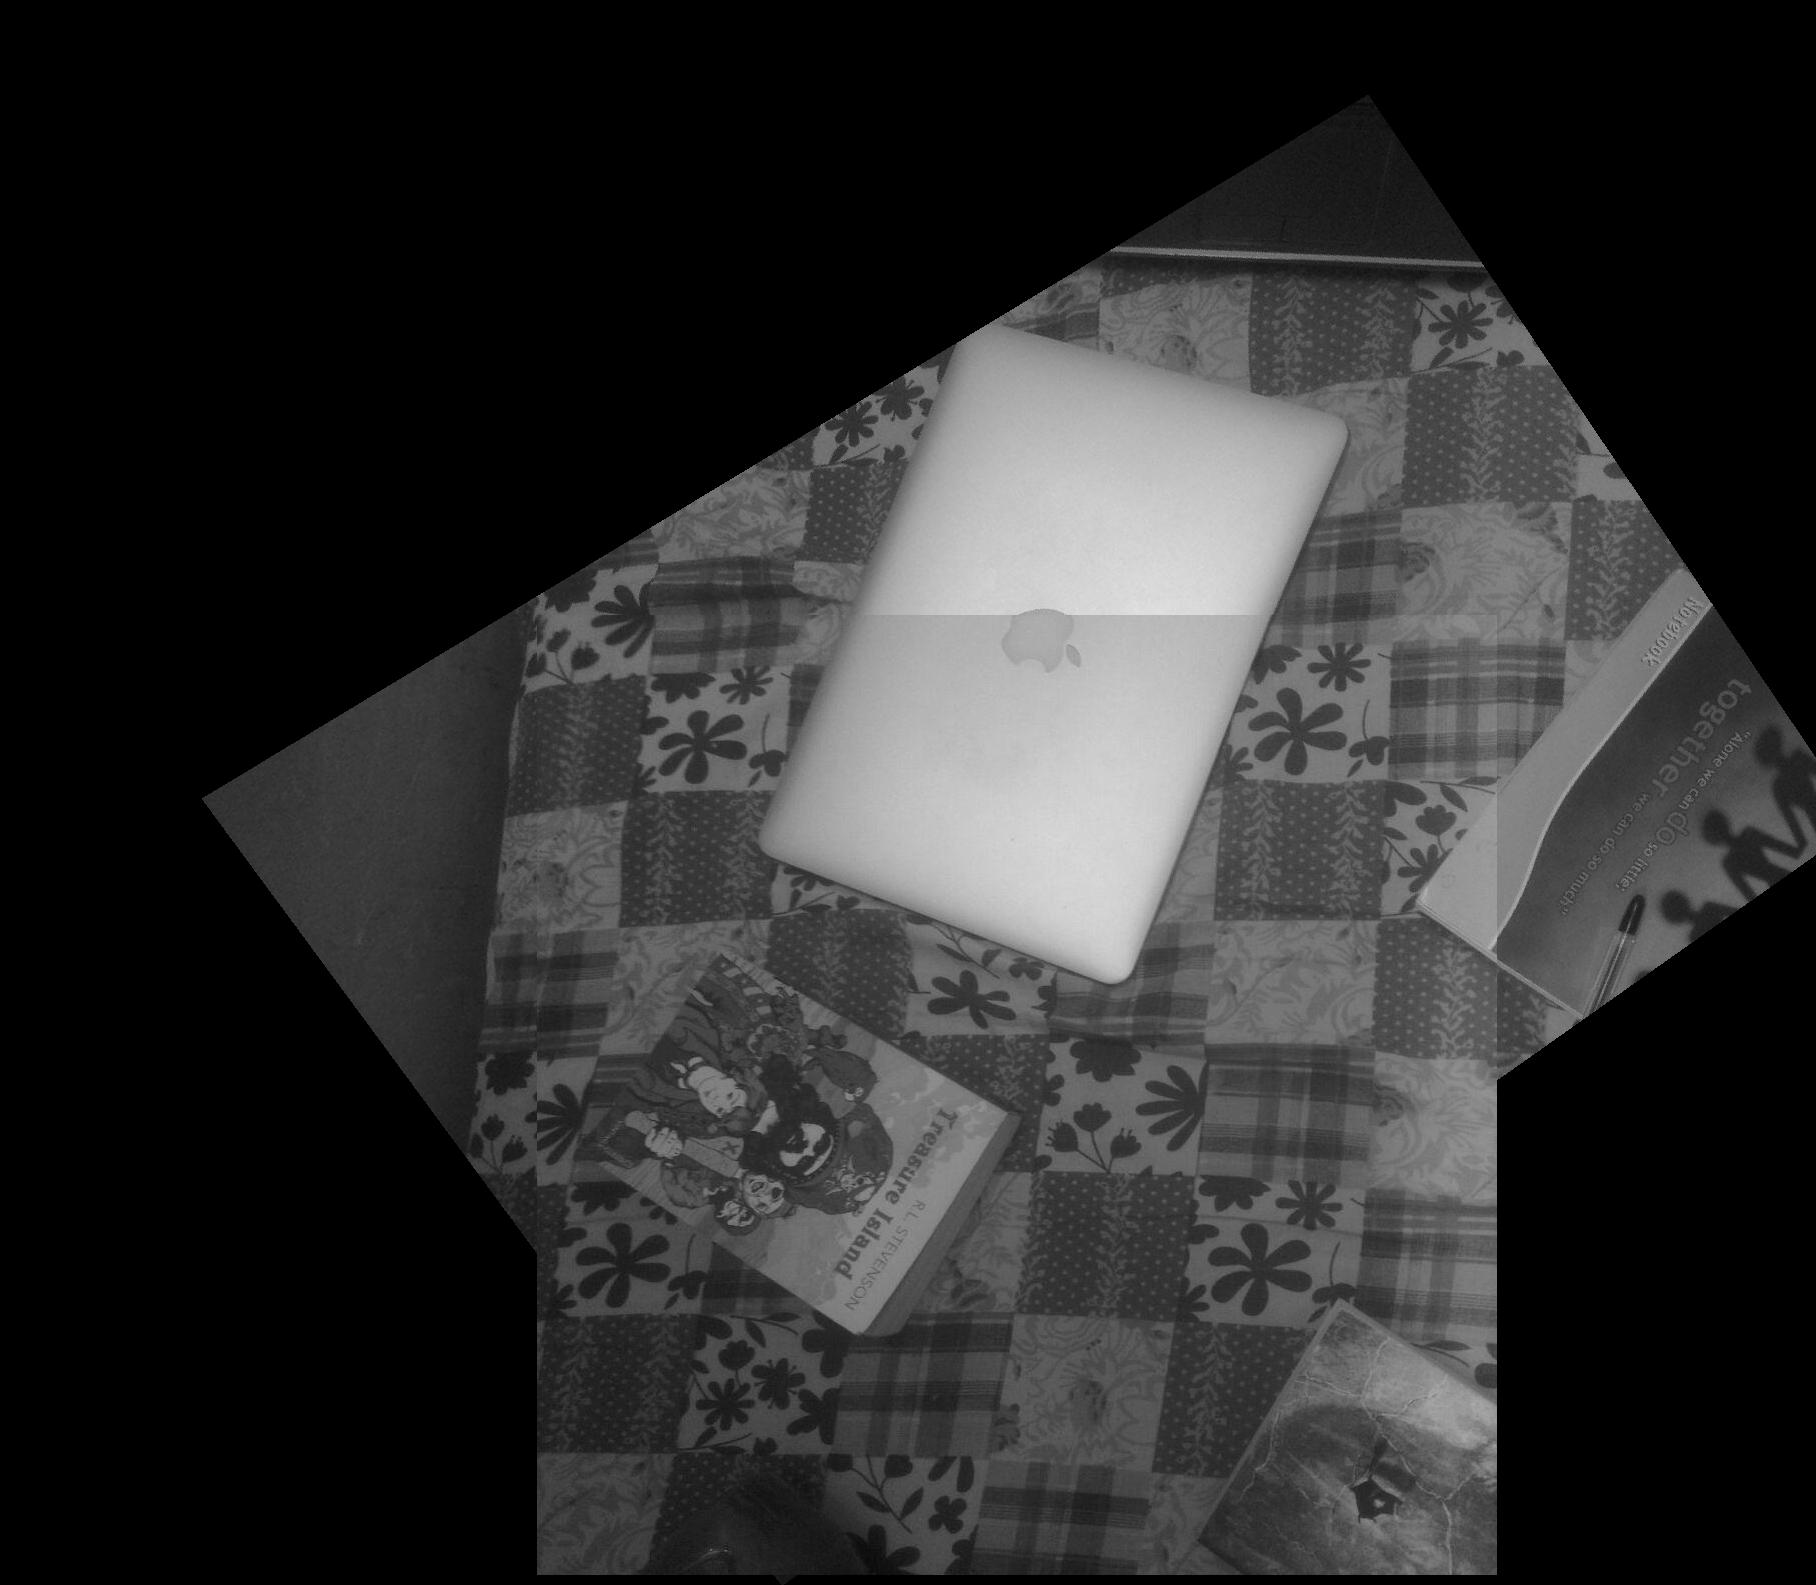
\includegraphics[width=3.5in]{new_result.jpg} }}%
	\caption{Mosaicing of another set of my images}
\end{figure}

\begin{figure}[!htb]
    \centering
    \subfloat[Image 1]{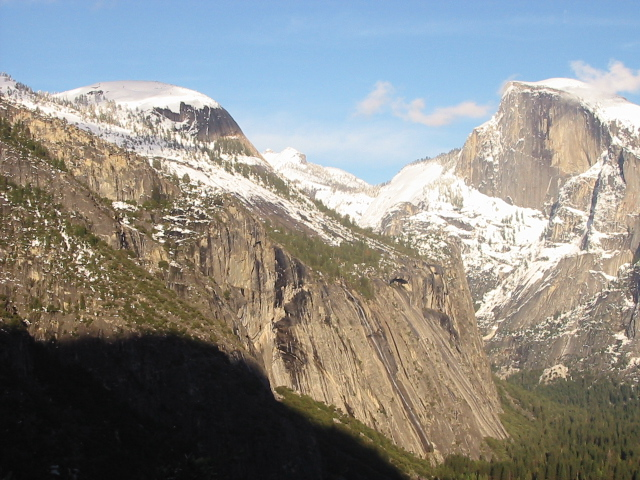
\includegraphics[width=2.5in]{yosemite1.jpg}}%
    \qquad
    \subfloat[Image 2]{{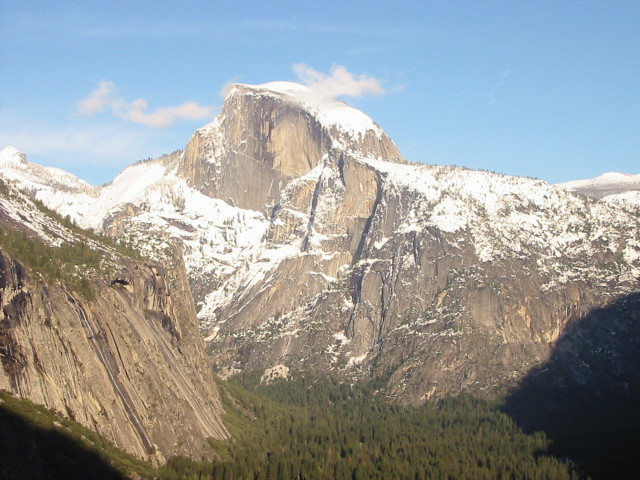
\includegraphics[width=2.5in]{yosemite2.jpg} }}%
	\qquad
	\subfloat[Image 3]{{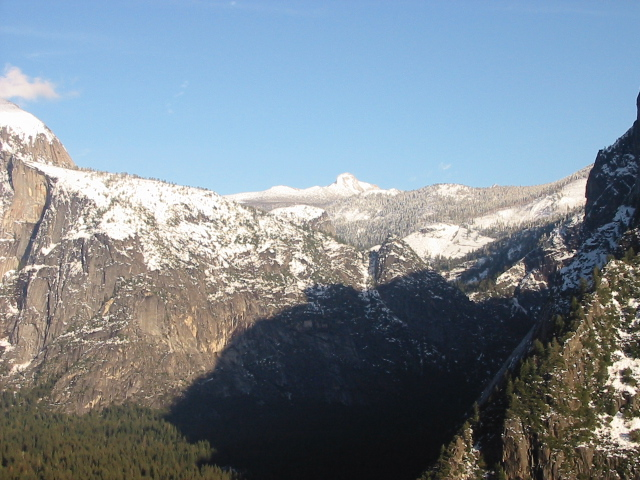
\includegraphics[width=2.5in]{yosemite3.jpg} }}%
	\qquad
	\subfloat[Image 4]{{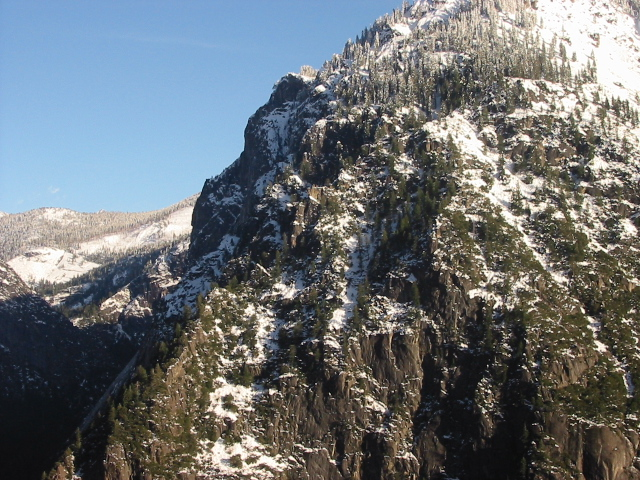
\includegraphics[width=2.5in]{yosemite4.jpg} }}%
	\qquad
	\subfloat[Mosaiced Image]{{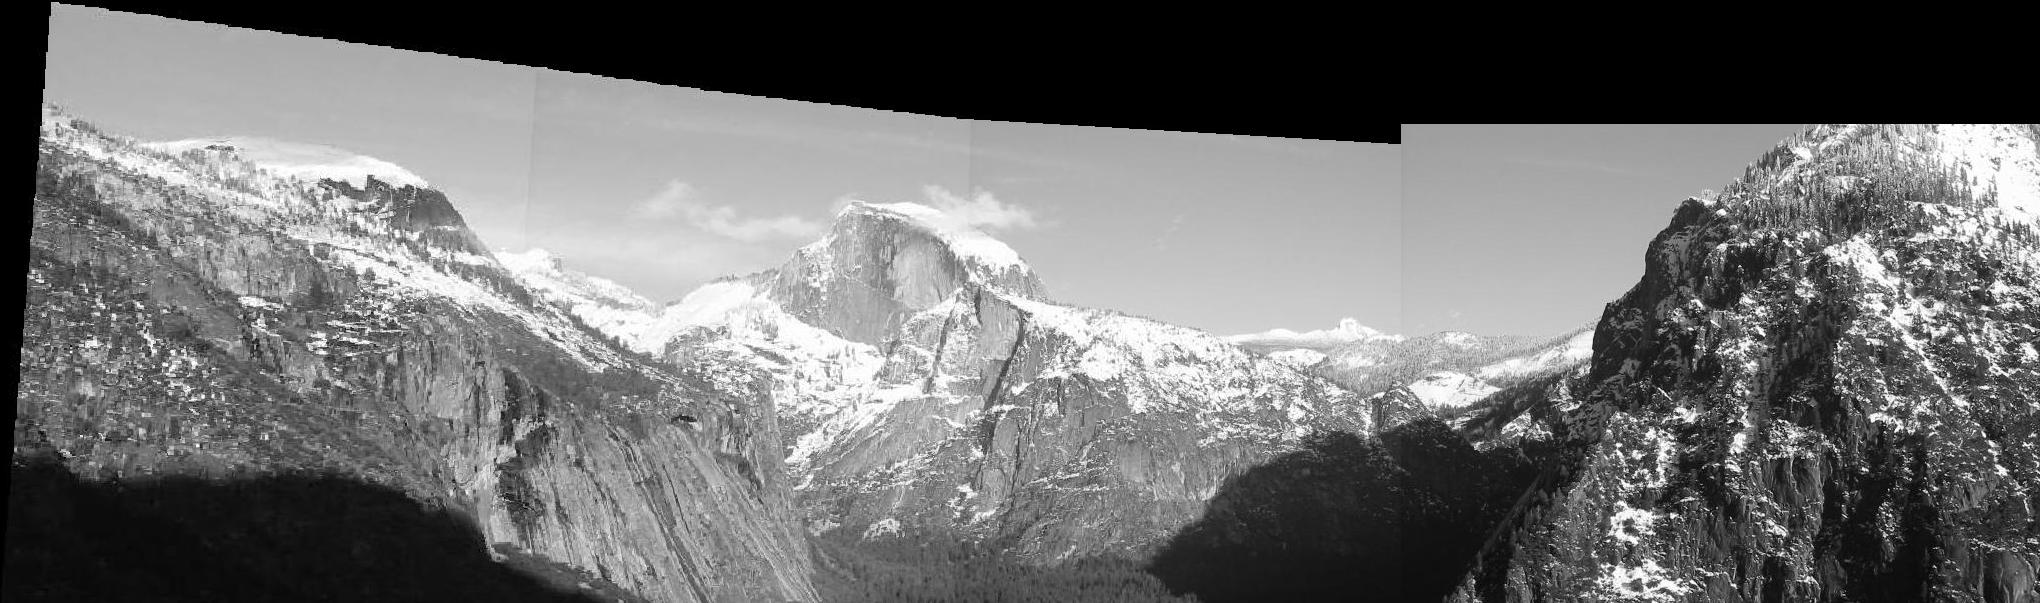
\includegraphics[width=6in]{yosemite_stiched.jpg} }}%
	\caption{Mosaicing of more than two photos of Yosemite}
\end{figure}
\end{itemize}
\item Here we will register a flash and a no-flash image pair using the joint entropy criterion we studied in class. Download the flash and no-flash images from \url{http:\\www.cse.iitb.ac.in/~ajitvr/CS763_Spring2015/HW2/ImageReg}. Convert both images to \sout{color} gray-scale. The flash image and the no-flash image have different image intensities at many places, and the no-flash image is distinctly noisier. Rotate the given no-flash image counter-clockwise by 28.5 degrees, translate it by -6 pixels in the X direction, and add Gaussian noise of standard deviation 5 (on a 0-255 scale). Note that the rotation must be applied about the center of the image. Set negative-valued pixels to 0 and pixels with value more than 255 to 255. Now perform a brute-force search to find the angle $\theta$ and translation $t_x$ to optimally align the modified no-flash image with the flash image, so as to minimize the joint entropy. The range for $\theta$ is between -60 and +60 in steps of 1 degree, and the range for $t_x$ should be between -12 and +12 in steps of 1. Compute the joint entropy using a bin-size of 10 for both intensities. Plot the joint entropy as a function of $\theta$ and $t_x$ using the surf and imshow commands of MATLAB. Also, determine a scenario where the images are obviously misaligned but the joint entropy is (falsely and undesirably) lower than the `true' minimum. Again, display the joint entropy as mentioned before. Include all plots in your report. \textsf{[7 points]} 
\begin{itemize}
\item[Ans.]
Please refer to figure 4 for relevant plots. Original Translation= -6\newline Original Rotation=$28.5^0$.
The minimum joint entropy point is $(t_x,\theta)=(6,-28)$.

When the translation is large, we don't get proper minimal joint entropy as there's little overlap between the two figures, As an example shown in the figure 4, we've rotated image by $28.5^0$ and translateed by $-100$ pixels and the plotted joint entropy. We notice that the minimum joint entropy on boundary points while it is supposed to occur at $100,-28^0$.
\begin{figure}[!htb]
    \centering
    \subfloat[Original Image]{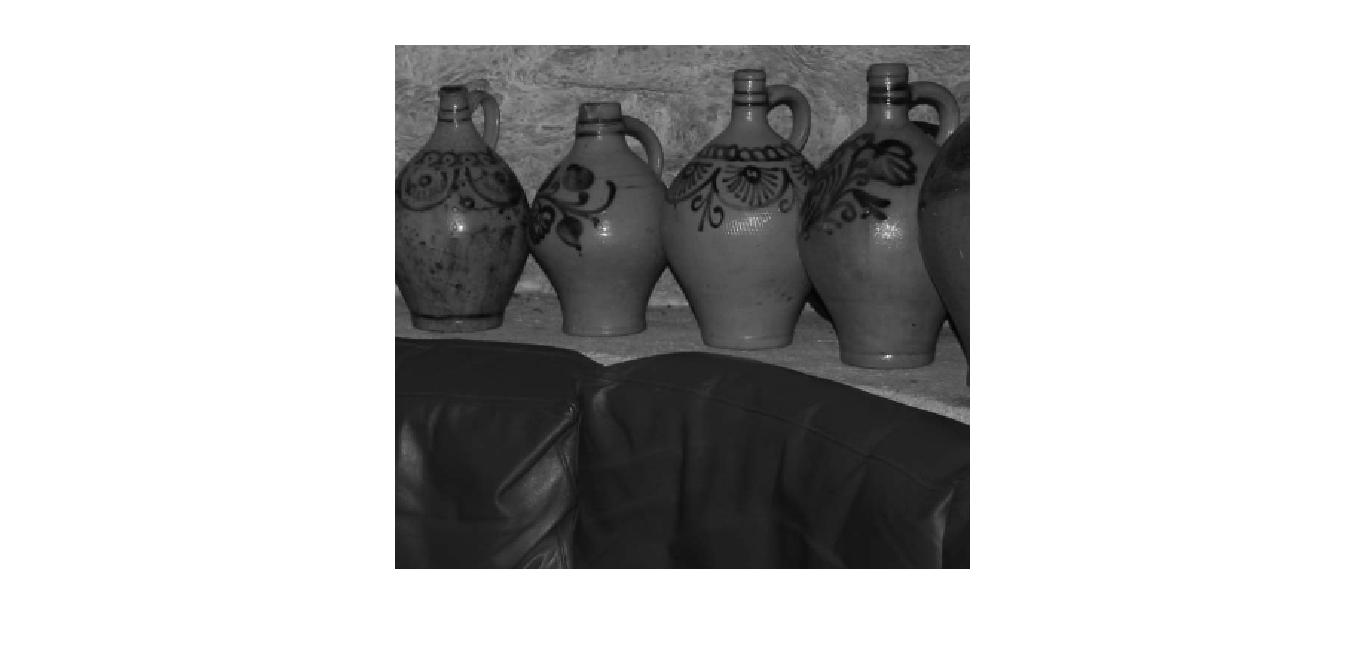
\includegraphics[width=2.5in]{1_Original.jpg}}%
    \qquad
    \subfloat[Misaligned Image]{{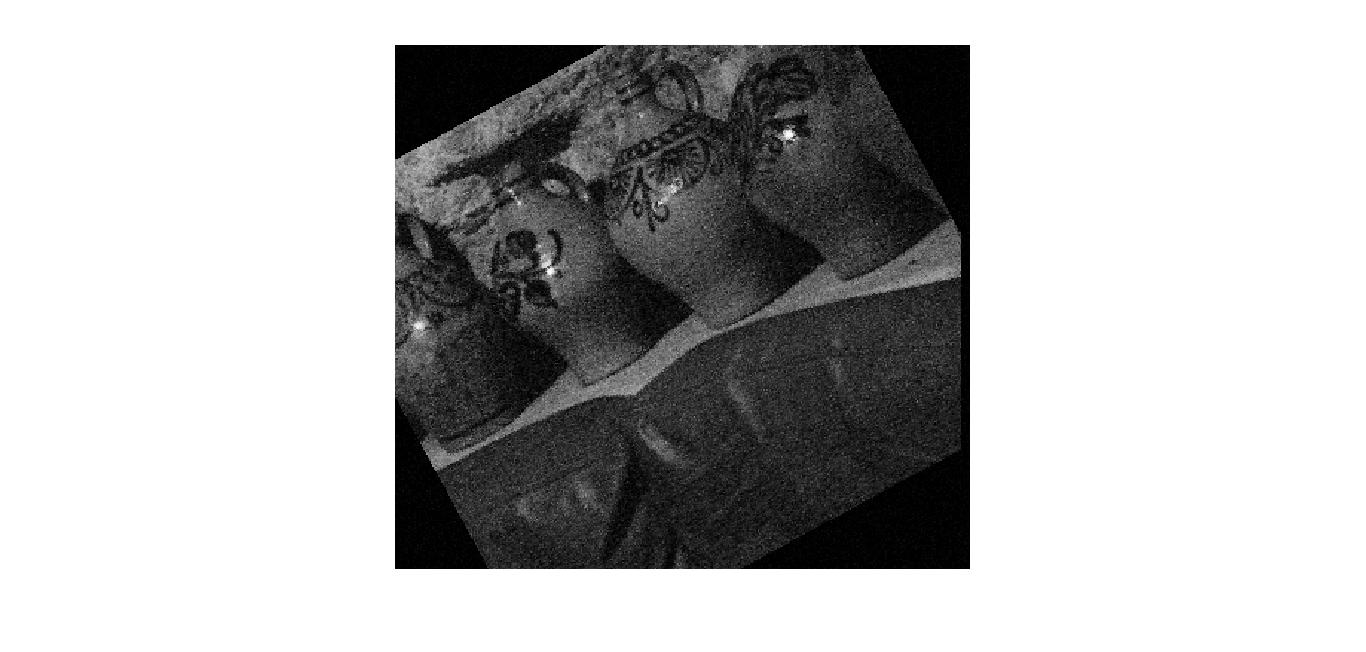
\includegraphics[width=2.5in]{2_MisAligned.jpg} }}%
	\qquad
	\subfloat[Realigned Image]{{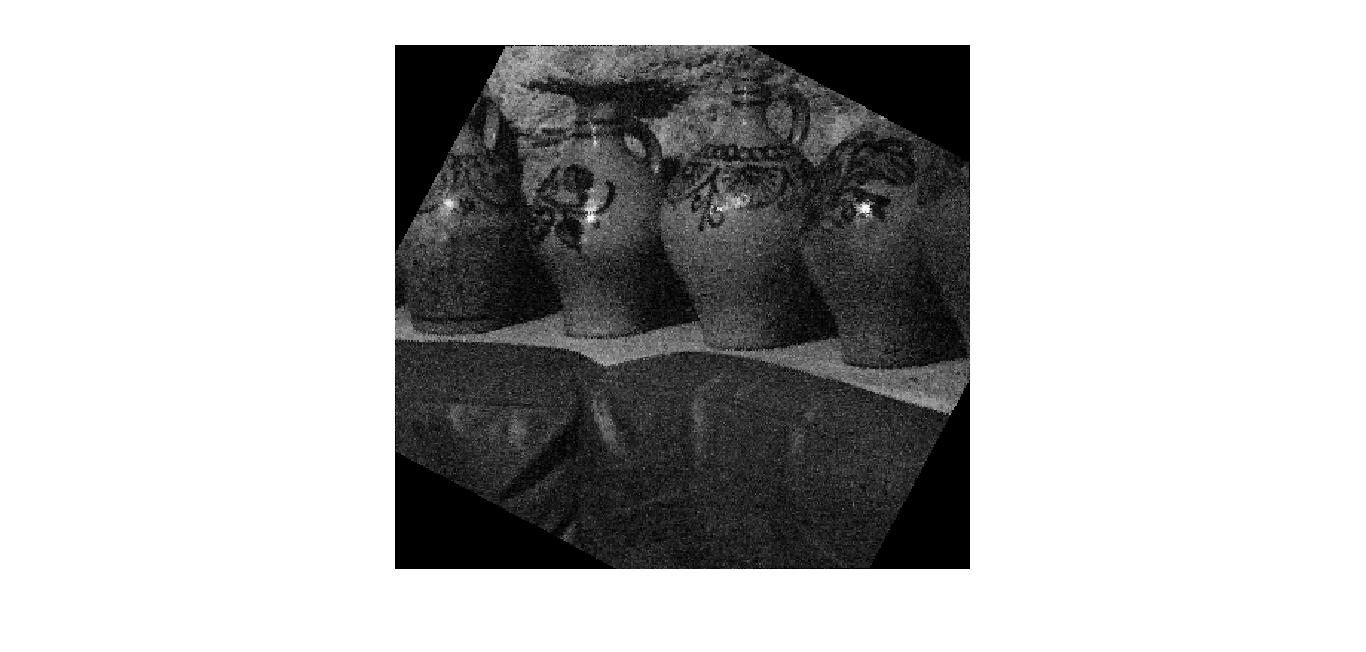
\includegraphics[width=2.5in]{3_ReAligned.jpg} }}%
	\qquad
	\subfloat[Joint Entropy surface plot]{{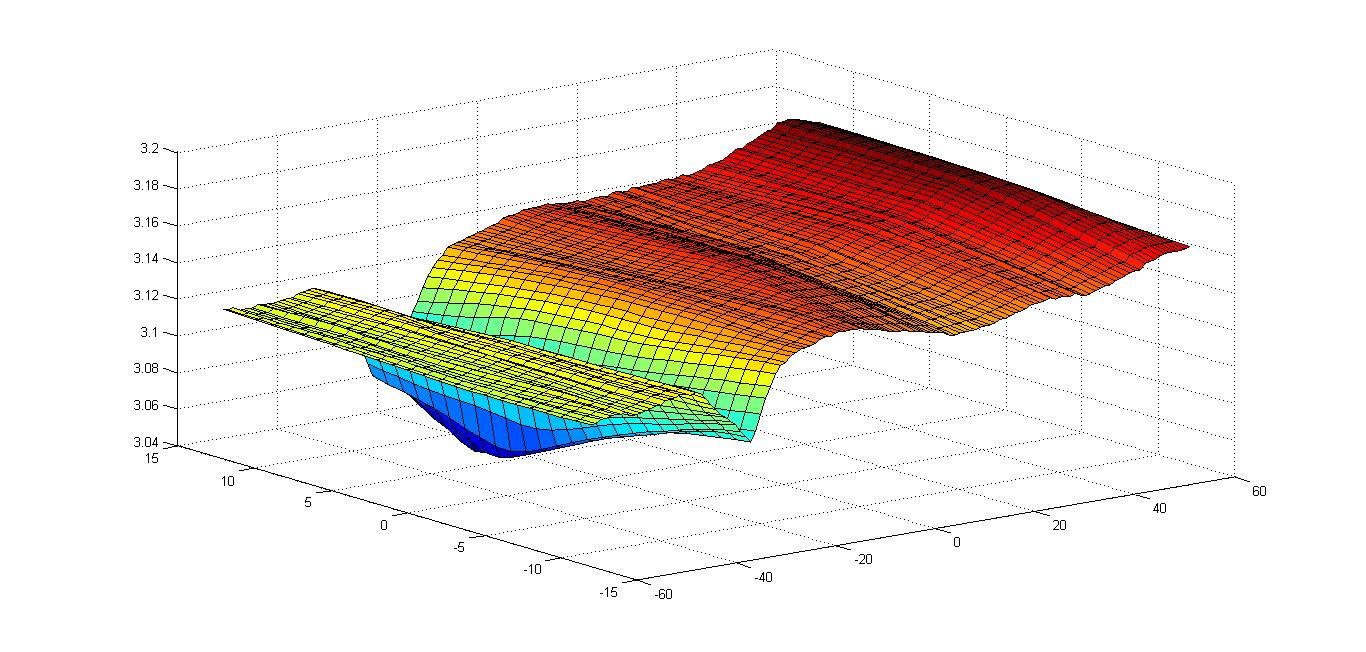
\includegraphics[width=5in]{surf.jpg} }}%
	\qquad
	\subfloat[Misaligned surface plot]{{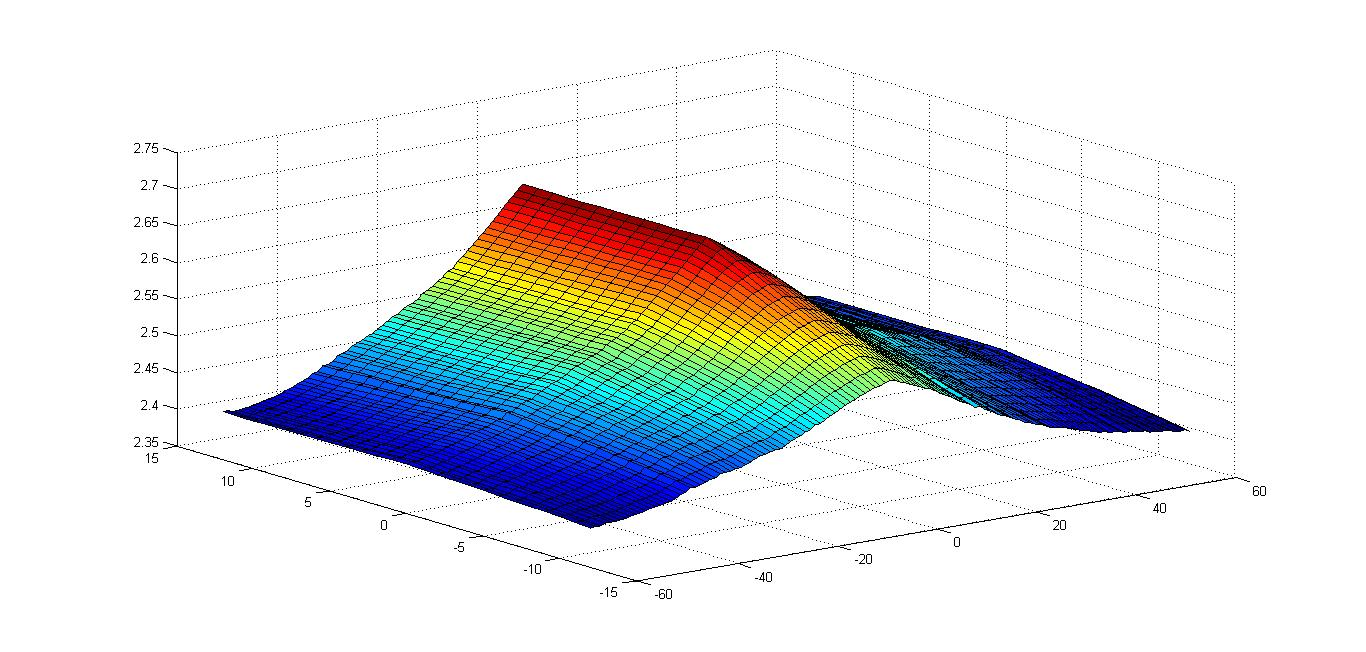
\includegraphics[width=5in]{surf_bad.jpg} }}%
	\caption{}
\end{figure}

\end{itemize}

\end{enumerate}
\end{document}